\chapter{``Natural'' proof strategies and complexity measures}

The lower bounds presented in \autoref{chap:gen-ckt} proceeded by first identifying a \emph{weakness} of the model, and exploiting it in an explicit manner. 
More concretely, \autoref{sec:Kalorkoti} presents a promising strategy that could be adopted to prove lower bounds for various models of arithmetic circuits. 
The crux of the lower bound was the construction of a good map $\Gamma$ that assigned a number to every polynomial. 
The map $\CM{Kal}$ was useful to show a lower bound in the sense that any $f$ computable by a \emph{small} formula had \emph{small} $\CM{Kal}(f)$. 
In fact, all subsequent lower bounds in arithmetic circuit complexity have more or less followed a similar template of a ``natural proof''. 
More concretely, all the subsequent lower bounds we shall see would essentially follow the outlined plan.  

\begin{quote}
{\bf Step 1 (normal forms)} For every circuit in the circuit class $\mathcal{C}$ of interest, express the polynomial computed as a \emph{small sum of simple building blocks}. 
\end{quote}

For example, every $\Sigma\Pi\Sigma$ circuit is a \emph{small} sum of \emph{products of linear polynomials} which are the building blocks here. 
In this case, the circuit model naturally admits such a representation but we shall see other examples with very different representations as sum of building blocks. 

\begin{quote}
{\bf Step 2 (complexity measure)} Construct a map $\Gamma: \F[x_1,\dots, x_n] \rightarrow \Z_{\geq 0}$ that is \emph{sub-additive} i.e. $\Gamma(f_1 + f_2)\leq \Gamma(f_1) + \Gamma(f_2)$.
\end{quote}

In most cases, $\Gamma(f)$ is the rank of a large matrix whose entries are linear functions in the coefficients of $f$. 
In such cases, we immediately get that $\Gamma$ is sub-additive. 

The strength of the choice of $\Gamma$ is determined by the next step. 

\begin{quote}
{\bf Step 3 (potential usefulness)} Show that if $B$ is a \emph{simple building block}, then $\Gamma(B)$ is \emph{small}.
Further, check if $\Gamma(f)$ for a \emph{random polynomial} $f$ is large (potentially). 
\end{quote}

This would suggest that if any $f$ with large $\Gamma(f)$ is to be written as a sum of $B_1 + \dots + B_s$, then sub-additivity and the fact that $\Gamma(B_i)$ is small for each $i$ and $\Gamma(f)$ is large immediately imply that $s$ must be large. 
This implies that the complexity measure $\Gamma$ does indeed have a potential to prove a lower bound for the class. 
The next step is just to replace the \emph{random polynomial} by an explicit polynomial. 

\begin{quote}
{\bf Step 4 (explicit lower bound)} Find an explicit polynomial $f$ for which $\Gamma(f)$ is large. 
\end{quote} 

These are usually the steps taken in almost all the known arithmetic circuit lower bound proofs. 
The main ingenuity lies in constructing a useful complexity measure, which is really to design $\Gamma$ so that it is small on the \emph{building blocks}. \\

Of course, there could potentially be lower bound proofs that do not follow the road-map outlined. 
For instance, it could be possible that $\Gamma$ is not small for a random polynomial, but specifically tailored in a way to make $\Gamma$ large for the $\Perm_n$. 
Or perhaps $\Gamma$ need not even be sub-additive and maybe there is a very different way to argue that all polynomial in the circuit class have small $\Gamma$. 
However, this has been the road-map for almost all lower bounds so far (barring very few exceptions). \\

In this chapter, we outline a few commonly used complexity measures and the typical context in which they are applied. 

\section{Sparsity}

The simplest example of a complexity measure is just the number of nonzero monomials in $f$. Clearly, this would yield lower bounds for circuits such as $\Sigma\Pi$ circuits (which can only compute sparse polynomials). But we shall see several non-trivial applications of sparsity as the complexity measure later on in the survey, especially in settings dealing with \emph{monotone} computation. 

\section{Dimension of partial derivatives}

Let $f(x_1,\ldots, x_n)$ be an $n$-variate, degree-$d$ polynomial. For a parameter $k$, we can define 
\[
\CM{PD}_k(f) = \dim \partial^{=k}(f).
\]
That is, consider the set of all $k$-th order partial derivatives of $f$ as a set of vectors and define $\CM{PD}_k(f)$ to be the dimension of their span. 

This can also be thought of as the rank of a matrix $M(f)$ where each row corresponds to a partial derivative, each column corresponds to a monomial, and the rows are just the coefficient vector of the specific partial derivative of $f$ written down. 

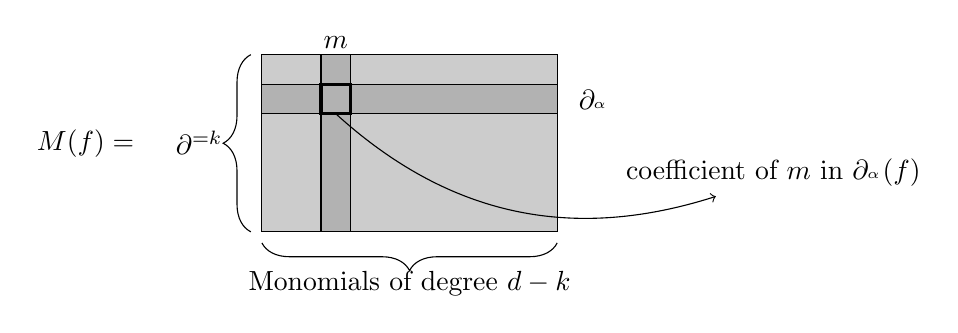
\begin{tikzpicture}[scale=0.75]
\draw[fill=black!20] (0,0) rectangle (5,3);

\draw[decorate,decoration={brace,amplitude=10pt,raise=4pt},yshift=0pt]
(0,0) -- (0,3);
\node[anchor=east] at (-2,1.5) {$M(f) = $};
\node[anchor=east] at (-0.5,1.5) {$\partial^{=k}$};
\draw[decorate,decoration={brace,amplitude=10pt,mirror, raise=4pt},yshift=0pt] 
(0,0) -- (5,0);
\node[anchor=north] at (2.5,-0.5) {Monomials of degree $d - k$};

\draw[fill=black!30] (1,0) rectangle (1.5,3);
\node at (1.25,3.2) {$m$};

\draw[fill=black!30] (0,2) rectangle (5,2.5);
\node[anchor=west] at (5.2,2.2) {$\partial_{\vecx^\alpha}$};

\draw[very thick] (1,2) rectangle (1.5,2.5);

\node[anchor=west] at (6,1) {coefficient of $m$ in $\partial_{\vecx^\alpha}(f)$}
edge[<-,bend left] (1.25,2);
\end{tikzpicture}

This measure has been very effective in giving lower bounds for depth-$3$ powering circuits, homogeneous depth-$3$ circuits etc. 

\subsection{An instructive example: depth-3 powering circuits}

A $\Sigma\!\wedge\!\Sigma$ circuit of size $s$ computes a polynomial of the form $f = \ell_1^{d_1} + \dots + \ell_s^{d_s}$ where each $\ell_i$ is a linear polynomial over the $n$ variables.\footnote{such circuits are also called \emph{diagonal depth-$3$ circuits} in the literature}

In this setting, the \emph{building blocks} are terms of the form $\ell^d$. 
The dimension of partial derivatives is very well suited for this setting.

\begin{observation}\label{obs:low-rank-sps-rank}
Any $k$-th order partial derivative of $\ell^d$ is a constant multiple of $\ell^{d-k}$. 
\end{observation}

Hence, if $f = \ell_1^d + \cdots + \ell_s^d$, then $\partial^{=k}(f)$ is spanned by $\setdef{\partial^{=k}(\ell_i^d)}{i\in [s]}$. Therefore, $\CM{PD}_k(f) \leq s$. 

For a random polynomial $f$, we should be expecting $\CM{PD}_k(f)$ to be $\binom{n+k}{k}$ as there is unlikely to be any linear dependencies among the partial derivatives. 
Hence, all that needs to be done is to find an explicit polynomial with large $\CM{PD}_k$. 

If $f = x_1 \cdots x_n$, then we can clearly see that the space of $k$-th order partial derivatives is spanned by ``sub-monomials'' of degree $n-k$. Therefore, 
\[
\CM{PD}_k(x_1 \cdots x_n) \geq \binom{n}{k}
\]
By setting $k = n/2$, we immediately get the following lower bound. 

\begin{corollary}
  If $x_1\cdots x_n = \ell_1^n + \cdots + \ell_s^n$, then $s \geq 2^{\Omega(n)}$. 
\end{corollary}

If we consider $\Det_n$ or $\Perm_n$, then any partial derivative of order $k$ is just an $(n-k)\times(n-k)$ minor. 
Also, these minors consist of disjoint sets of monomials and hence are linearly independent. 
Hence, $\CM{PD}_k(\Det_n) = \binom{n}{k}^2$. 
Choosing $k = n/2$, we immediately get that any $\Sigma\!\wedge\!\Sigma$ circuit computing $\Det_n$ or $\Perm_n$ must be of size $2^{\Omega(n)}$. 

\begin{exercise}
The above lower bound can be extended to \emph{rank-$r$ $\Sigma\Pi\Sigma$ circuit} that computes a polynomial of the form 
$$
f \spaced{=}  T_1 \;+\; \dots \;+\; T_s
$$
where each $T_i = \ell_{i1}\dots \ell_{id}$ is a product of linear polynomials such that $\dim\inbrace{\ell_{i1},\dots, \ell_{id}}\leq r$.

\medskip

Use the partial derivative measure and prove a lower bound for rank-$r$ $\Sigma\Pi\Sigma$ circuits for $r = O(1)$. 

\medskip

How large can you make $r$ and still get a non-trivial lower bound? 
\end{exercise}

\section{Dimension of the communication matrix}

Consider a partition of the underlying set of variables $X$ into two parts $X = Y \sqcup Z$. For this partition, we define the following ``partition matrix'' for any polynomial $f(X)$ given as follows:

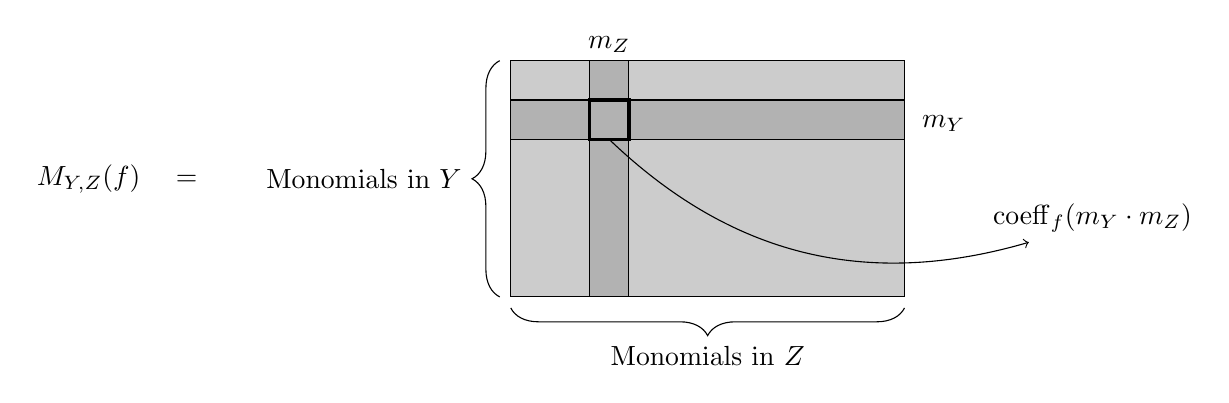
\begin{tikzpicture}
\node at (-5,1.5) {$M_{Y,Z}(f) \quad= $};
\draw[fill=black!20] (0,0) rectangle (5,3);

\draw[decorate,decoration={brace,amplitude=10pt,raise=4pt},yshift=0pt]
(0,0) -- (0,3);
\node[anchor=east] at (-0.5,1.5) {Monomials in $Y$};
\draw[decorate,decoration={brace,amplitude=10pt,mirror, raise=4pt},yshift=0pt] 
(0,0) -- (5,0);
\node[anchor=north] at (2.5,-0.5) {Monomials in $Z$};

\draw[fill=black!30] (1,0) rectangle (1.5,3);
\node at (1.25,3.2) {$m_Z$};

\draw[fill=black!30] (0,2) rectangle (5,2.5);
\node at (5.5,2.2) {$m_Y$};

\draw[very thick] (1,2) rectangle (1.5,2.5);

\node[anchor=west] at (6,1) {$\mathrm{coeff}_f(m_Y \cdot m_Z)$}
edge[<-,bend left] (1.25,2);
\end{tikzpicture}

Let $\CM{CM}_{Y,Z}(f) = \rank M_{Y,Z}(f)$. This measure has been quite effective in proving lower bounds in multilinear and non-commutative settings. 

\subsection{An instructive example: read-once oblivious ABPs}

A \emph{read-once oblivious ABP} (ROABP) (in the order $x_1,\ldots, x_n$) is a branching program that computes a polynomial of the following form:
\[
f = A_1(x) \cdots A_n(x_n)
\]
where $A_1(x)$ is a $1 \times w_1$ matrix, $A_n(x_n)$ is a $w_{n-1} \times 1$ matrix and each $A_i(x_i)$ is a $w_{i-1} \times w_i$ matrix. This can be thought of as an ABP with $n+1$ layers, and each $A_i$ capturing the bipartite adjacency matrix between layer $i-1$ and $i$. 

All entries in $A_i(x_i)$ are just univariates in $x_i$. The degree of the ROABP is defined as the maximum degree of any entry in the $A_i$'s, and the size of the ROABP is the sum of the $w_i$'s. \\

When dealing with ROABPs, we can split the computation by ``cutting'' the ABP at any layer $i$ to obtain
\[
f = \sum_{i=1}^{w_i} g_i(x_1,\ldots, x_i) \cdot h_i(x_{i+1}, \ldots, x_n)
\]
and this decomposition makes the rank of the communication matrix perfectly suited to prove lower bounds. 

\begin{observation}
Let $X = Y \sqcup Z$. Suppose $f(X) = g(Y) \cdot h(Z)$ for some polynomials $g,h$. Then $\CM{CM}_{Y,Z}(f) = 1$. 
\end{observation}
\begin{proof}
Follows immediately from noticing that $M_{Y,Z}(f)$ is just the outer-product of the coefficient vector of $g$ and $h$ respectively since $\coeff_{Y^aZ^b}(f) = \coeff_{Y^a}(g) \cdot \coeff_{Z^b}(h)$. 
\end{proof}

\begin{corollary}
For each $i \in [n]$, any ROABP computing $f$ (in the order $x_1,\ldots, x_n$) must satisfy $w_i \geq \CM{CM}_{Y,Z}(f)$ where $Y = \set{x_1,\ldots, x_i}$ and $Z = \set{x_{i+1}, \ldots, x_n}$. 
\end{corollary}

The polynomial $f(y_1,\ldots, y_m, z_1,\ldots, z_m) = (y_1 z_1 + 1) \cdots (y_m z_m + 1)$ has $M_{Y,Z}(f)$ as just the identity matrix and thus $\CM{CM}_{Y,Z}(f) = 2^m$. This immediately says that any ROABP for $f$ in the order $y_1,\ldots, y_m, z_1,\ldots, z_m$ must have size $2^{\Omega(n)}$. 

\section{Variants of these measures}

Over the years, there have been several variants over these measures that have been immensely successful. These have been by adding monomials shifts to the space of polynomials and then considering their span (such as \emph{shifted partial derivatives}), or projecting the set of rows / columns to some natural subsets (projected shifted partials derivatives, or affine projection of partial derivatives), or considering ``random'' partition of variables etc.

In the course of the survey we will see various examples of these variants. 